\documentclass{article}
\usepackage[utf8]{inputenc}
\usepackage{graphicx}
\usepackage{float}
\usepackage{amsmath}
\usepackage{amssymb}
\usepackage{amsthm}
\usepackage{commath}

\graphicspath{{figures/}}

\newtheorem{question}{Question}
\newcommand{\RR}{\mathbb{R}}
\newcommand{\NN}{\mathbb{N}}
\newcommand{\ZZ}{\mathbb{Z}}
\newcommand{\T}[1]{#1^{\top}}
\newcommand{\kth}[2][k]{#2^{(#1)}}
\DeclareMathOperator{\diag}{diag}
\DeclareMathOperator*{\argmin}{arg min}
\DeclareMathOperator{\Span}{span}
\DeclareMathOperator{\proj}{proj}

\title{Hints for OCS Questions}
\author{Julian Wolf \and Philipp Gabler}


\begin{document}
\maketitle

\section{Basics}

%%%%%%%%%%%%%%%%%%%%%%%%%%%%%%%%%%%%%%%%%%%%%%%%%%%%%%%%%%% 
\begin{question}
  What is the definition of a general mathematical optimization problem?  Give an example and
  explain the notion of an objective function, a constraint set, an optimal solution and the
  definition of the level sets of a function.
\end{question}
Draw level lines and arrows
\begin{itemize}
\item objective function is the function we want to minimize
\item constraint set is a set of functions
\item optimal solution: find $f(x^*) \leq f(x), \forall x \in X$
\item level set: compareable to level lines of terrain, convex function $=>$ convex level set (but
  there are non convex fct with convex level sets),
\end{itemize}

%%%%%%%%%%%%%%%%%%%%%%%%%%%%%%%%%%%%%%%%%%%%%%%%%%%%%%%%%%% 
\begin{question}
  Explain nonlinear programming, linear programming, quadratic programming, convex programming and
  give examples. What is the definition of a convex set and a convex function? Give examples for
  convex sets and convex functions.
\end{question}
\begin{itemize}
\item \textbf{Linear}: Objective Function and Constraints may only be linear
  $min\ c^Tx, s.t.\ Ax \leq b, x \geq 0$\\
  Polynomial solvable
\item \textbf{Non Linear}: Objective Function and Constriants may  be non linear
  $min\ \frac{1}{2} x^TQx + c^Tx, s.t.\ Ax \leq b, Ex = d$\\
  Q symmetrical and pos. definite, polynomial solvable
\item \textbf{Quadratic}: objective function is quadratic, constraints are linear	
  $min_{x \in \mathbb{R}}\ f_0(x) \texttt{ (objective)},$\\
  $s.t.\ f_i(x) \leq i=0..m \texttt{ (contraints)}$\\
  polynomial time
\item \textbf{convex set}: 
  $\alpha x + (1 - \alpha)y \ in X, \forall x, y \in X, \alpha \in [0, 1]$
\item \textbf{convex fct}:
  $f(\alpha x + (1 - \alpha)y) \leq \alpha f(x) + (1 - \alpha)f(y) , \forall x, y \in X, \alpha \in
  [0, 1]$
\end{itemize}

%%%%%%%%%%%%%%%%%%%%%%%%%%%%%%%%%%%%%%%%%%%%%%%%%%%%%%%%%%% 
\begin{question}
  What is the difference between local and global minima. Give examples.  Give the first order
  necessary condition of optimality and prove it. What is the second order necessary condition of
  optimality? Show that for differentiable convex functions, the first order necessary condition of
  optimality becomes sufficient.
\end{question}
\begin{itemize}
\item When hessian is strictly positive, it is a strict global maximum
\item \textbf{unconst Local minimum:}
  $f(x^*) \leq f(x), \forall x \texttt{ with } || x - x^* || \leq \varepsilon$
\item \textbf{unconst global minimum:} $f(x^*) \leq f(x), \forall x \in \mathbb{R}$
\end{itemize}

\begin{figure}[H]
  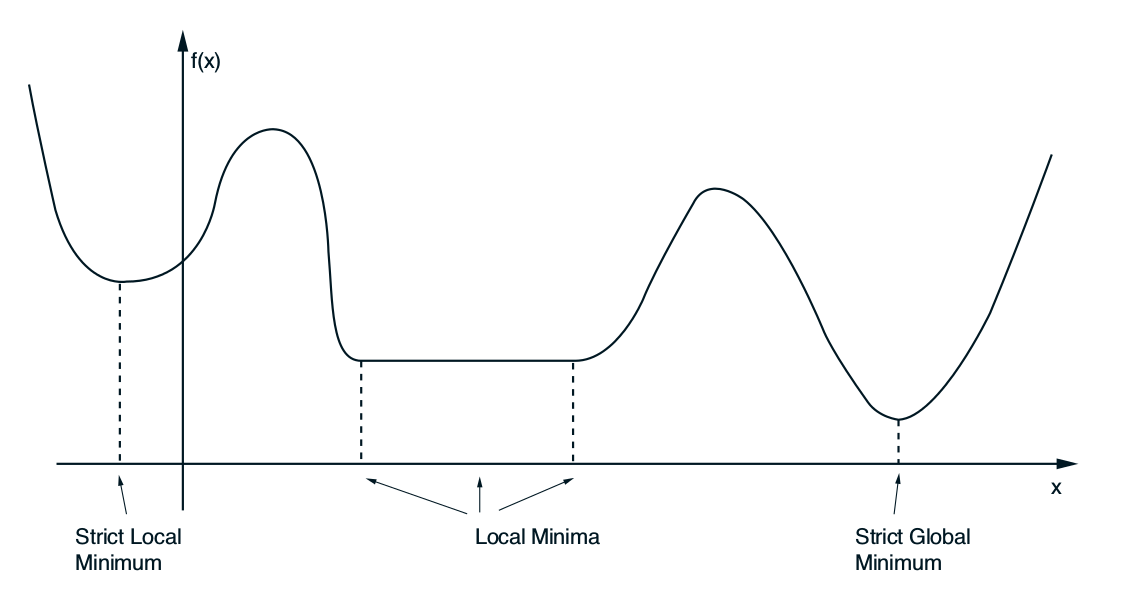
\includegraphics[width=\textwidth]{loc_glob_min.png}
  \caption{Local/Global minimas\label{fig:min}}
\end{figure}

\section{Gradient Methods, Optimality}

%%%%%%%%%%%%%%%%%%%%%%%%%%%%%%%%%%%%%%%%%%%%%%%%%%%%%%%%%%% 
\begin{question}
  Discuss the optimality conditions for a quadratic optimization problem of the form
  \[ \min_x \frac{1}{2} \T{x} Q x - \T{b} x.
  \]
  When is this problem convex and what does convexity imply? Give a simple example in 2D showing
  different realizations of \(Q\).
\end{question}
\begin{itemize}
\item If positive and negative Eigenvalues, we can not define convexity
\item First order necessessary optimality condition: $\nabla f(x^*) = 0$
\item Second order necessessary optimality condition: $\nabla^2 f(x^*) $ is positive semi definite

  \begin{figure}[H]
    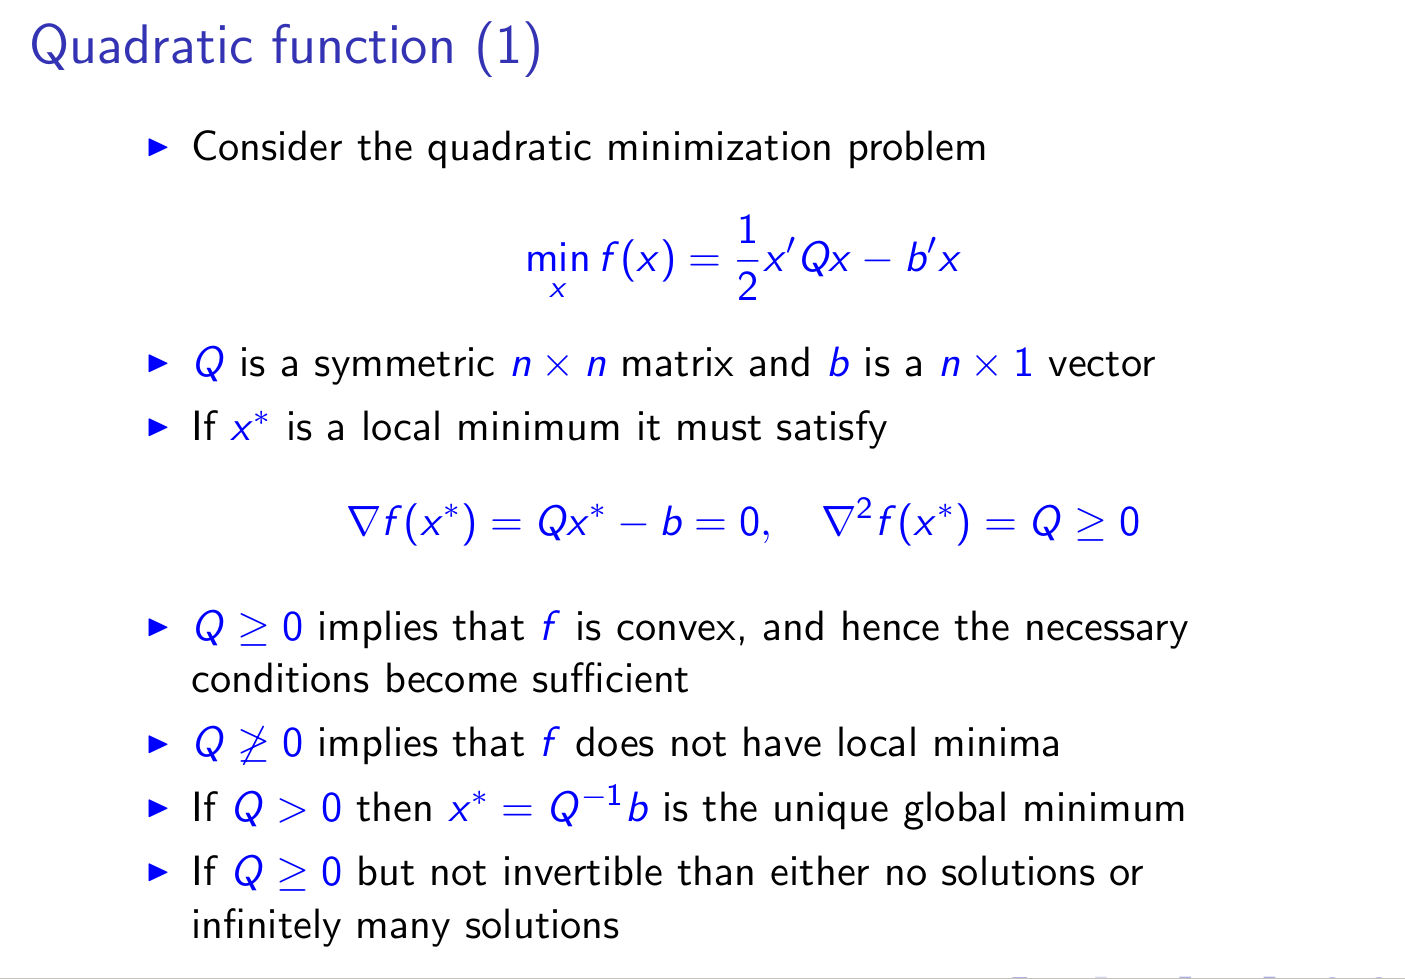
\includegraphics[width=\textwidth]{cond_quad_q.png}
    \caption{Different scenarios for Q\label{fig:cond_quad}}
  \end{figure}	
\end{itemize}

%%%%%%%%%%%%%%%%%%%%%%%%%%%%%%%%%%%%%%%%%%%%%%%%%%%%%%%%%%% 
\begin{question}
  What is a descent direction. Draw a simple example explaining the properties of a descent
  direction. Give the general form of a gradient method and show that
  \(\kth{d} = -\kth{D} \nabla f(x_k)\) with \(\kth{d}\) symmetric and positive definite is a descent
  direction.
\end{question}
\begin{itemize}
\item Descent direction: angle of step and derivation direction $< 90^\circ$
\item General form of gradient method: \\
  1. Choose an initial vector $x ^0 \in \mathbb{R}^n$\\
  2. Choose a descent direction $d^k$ that satisfies $\nabla f (x^k)'  d^k < 0$\\
  3. Choose a positive step size $\alpha^k$\\
  4. Compute the new vector as\\
  $x^{k+1} = x^k + \alpha^k d^k$\\
  5. Set $k = k + 1$ and goto 2
  \begin{figure}[H]
    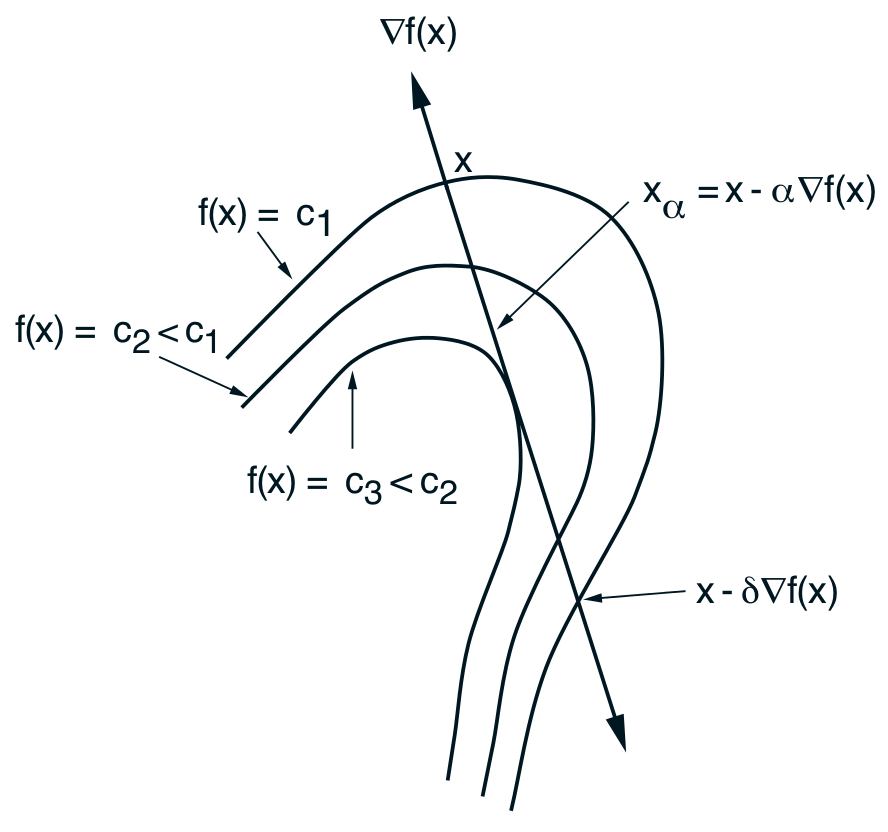
\includegraphics[width=\textwidth]{desc_dir.png}
    \caption{Simple descent direction\label{fig:desc_dir}}
  \end{figure}
\end{itemize}

%%%%%%%%%%%%%%%%%%%%%%%%%%%%%%%%%%%%%%%%%%%%%%%%%%%%%%%%%%% 
\begin{question}
  Give three different standard choices for descent directions based on choosing the scaling matrix
  \(\kth{D}\) and discuss their numerical performance. What is the Armijo step size selection
  rule? Draw an example explaining the set of acceptable step sizes.
\end{question}
$d^k = -D^k \nabla f (x^k )$
\begin{itemize}
\item Identity: $D^k = I$, = Gradient descent, zig zagging problem, very bad on Rosenbrock Fct
\item Hessian: $D^k = \nabla^2 f(x^k)$, = Newtons method, very fast convergence, very good on
  rosenbrock, unstable in despite of initial values (may diverge or find local maxima instead of
  minima), con: calculation of inverse of hessian - very expensive in large networks
\item Diagonal Hessian (approximation of Newton): $d_i^k \approx \left(
    \frac{\partial^2  f (x^k)}{(\partial x_i)^2}
  \right)^{-1}$, very bad performance on Rosenbrock, 
\item Gauss Newton method: Too complicated to remember, replace $D^k$ with non linear least square
  problem, even better performance on rosenbrock then newton, con: again calculation of inverse, but
  not of hessian
\item \textbf{Step size} $\alpha$: 
  \begin{itemize}
  \item \textbf{Minimization rule:} choose $\alpha$ such that $f(x + \alpha d)$ is minimized along
    $d$. Hard if $f$ is complicated
  \item \textbf{Limited minimization rule:} iterative: start small and increase size of $\alpha$
    until $f(x)$ is bigger then before, then choose the previous. Easy to implement
  \item \textbf{Armijo rule:} it is not sufficient that $f(x^{k+1}) < f(x^k)$, thus, the step sizes
    $\beta^ms$ for $m = 0,1,...$ are chosen such that the energy decrease is sufficiently large
    (dependent on derivation of $f(x)$, formula too complicated), or graphical:
    \begin{figure}[H]
      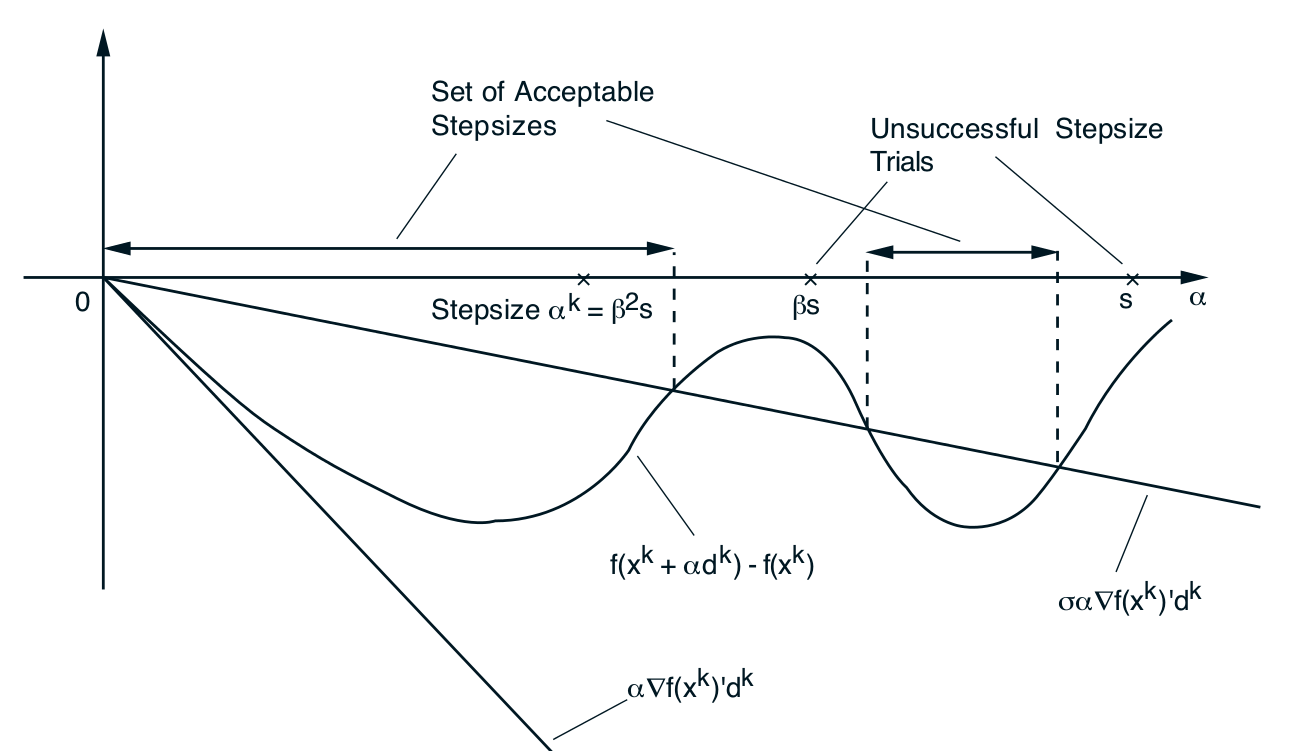
\includegraphics[width=\textwidth]{armijo.png}
      \caption{Graphical representation of the idea of Armijo\label{fig:desc_dir}}
    \end{figure}
    
  \end{itemize}
\end{itemize}

\section{Convergence}

%%%%%%%%%%%%%%%%%%%%%%%%%%%%%%%%%%%%%%%%%%%%%%%%%%%%%%%%%%% 
\begin{question}
  What is a Lipschitz continuous gradient, and what is the descent lemma?  Give the proof of the
  descent lemma.
\end{question}
\begin{itemize}

\item there exists a definite real number such that, for every pair of points on the graph of this
  function, the absolute value of the slope of the line connecting them is not greater than this
  real number
  
\item (There is something missing here)
  
\end{itemize}

%%%%%%%%%%%%%%%%%%%%%%%%%%%%%%%%%%%%%%%%%%%%%%%%%%%%%%%%%%% 
\begin{question}
  What is a rate of convergence? Explain linear, superlinear, and sublinear convergence and give
  examples.
\end{question}
\begin{itemize}
\item \textbf{Linear:} $\limsup_{k \rightarrow \infty} \frac{e(x^{k+1})}{e(x^k)}\leq \beta$ (blue line)
\item \textbf{superlinear:} $\limsup_{k \rightarrow \infty} \frac{e(x^{k+1})}{e(x^k)^p} < \infty$ (red line)
\item \textbf{sublinear:} $\limsup_{k \rightarrow \infty} \frac{e(x^{k+1})}{e(x^k)} = 1$ (black line)
\end{itemize}

\begin{figure}[H]
  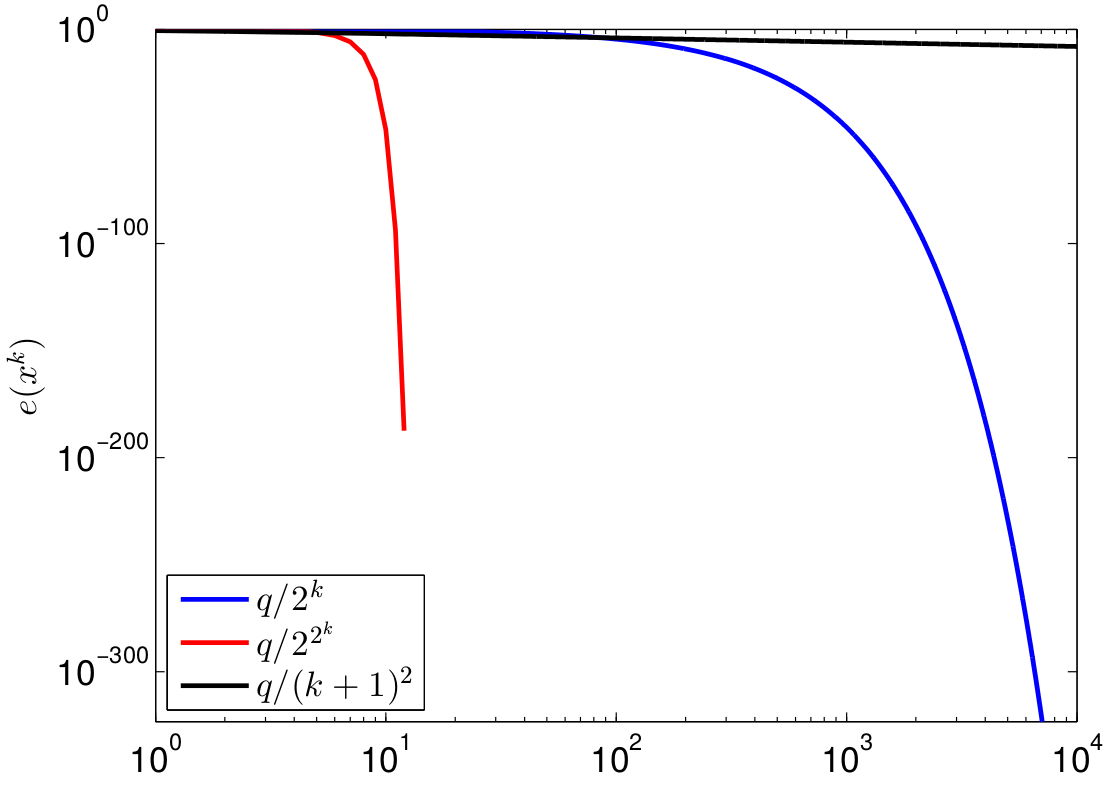
\includegraphics[width=10cm]{convergence.png}
  \caption{Graphical representation of linear, superinear and sublinear
    convergence \label{fig:desc_dir}}
\end{figure}

\section{Newton's method}

%%%%%%%%%%%%%%%%%%%%%%%%%%%%%%%%%%%%%%%%%%%%%%%%%%%%%%%%%%% 
\begin{question}
  Show that the plain form of Newton’s method can be derived from a second order Taylor
  approximation of the objective function. Show that Newton’s method is invariant with respect to an
  affine change of the coordinate system.
\end{question}
\begin{itemize}
\item $\tilde{g}(x, x^k) = g(x^k) + \nabla g(x^k)'(x - x^k)$
\item is affine: because the derivation of the function is independent to a move of constants?!?!?
\end{itemize}

\section{Least squares problems}

%%%%%%%%%%%%%%%%%%%%%%%%%%%%%%%%%%%%%%%%%%%%%%%%%%%%%%%%%%% 
\begin{question}
  What are linear (and nonlinear) least squares problems. Give an example.  What is the Gauss-Newton
  method and what is its relation to Newton’s method?
\end{question}
\textbf{Linear}:
\begin{itemize}
\item pointcloud, best fitting by polynomial equations
\item Solve least square problem to find optimal parameters
\item $\frac{1}{2}|| Ax - z ||^2$
\end{itemize} 
\textbf{Non-Linear:}
\begin{itemize}
\item Measure distance to beacons to get our own unkown location
\item non linear least squares problem
\item $min_x \frac{1}{2} \sum_{i = 1^m} (d_i - \sqrt{(x_i - p_1^i)^2 + (x_2 - p_2^i)^2})^2$
\end{itemize} 
\textbf{Gauss-Newton}:
\begin{itemize}
\item Uses $(\nabla g(x^k)\nabla g(x^k)')^{-1}$ instead of hessian
\item Approximates Current point with parabola and minimizes this subproblem (as plain Newton)
\end{itemize}
(check this shit out)

%%%%%%%%%%%%%%%%%%%%%%%%%%%%%%%%%%%%%%%%%%%%%%%%%%%%%%%%%%% 
\begin{question}
  What is a Kalman filter. How does it relate to an optimization problem?  What is an extended
  Kalman filter?
\end{question}
\begin{itemize}
\item incremental of gauss newton - incremental growing least squares estimate
\item example watertank: many measurements with noise - a very good and fast convergence to correct
  level is reached
\item extended Kalman Filter: input data behaves according to a function
\end{itemize}

\section{Accelerated gradient methods}

%%%%%%%%%%%%%%%%%%%%%%%%%%%%%%%%%%%%%%%%%%%%%%%%%%%%%%%%%%% 
\begin{question}
  What is the lower bound of first order methods on quadratic problems?  What is an optimal
  algorithm for quadratic problems?
\end{question}
\begin{itemize}
\item $Q$ positive definite: $\left(\frac{\sqrt{L/I}-1}{\sqrt{L/I} + 1}\right)^n || x^0  - x* ||$
\item $Q$ positive semidefinite: not motivated to write formula
\item Best method: conjugate gradient method (by Polyak) see next question
\end{itemize}

%%%%%%%%%%%%%%%%%%%%%%%%%%%%%%%%%%%%%%%%%%%%%%%%%%%%%%%%%%% 
\begin{question}
  Write down the conjugate gradient (CG) method and specialize the algorithm for solving a least
  squares problem of the form
  \[
    \min_x \frac{1}{2} \T{x} Q x - \T{b} x.
  \]
  What is the relation to solving linear system of equations?
\end{question}
\begin{itemize}
\item Motivation: converge faster the GD but avoid Newton overhead
\item Q-conjugate if: $d^i  Q d^j = 0, \forall i, j \texttt{ with } i \neq j$
\item Algorithm: Use Gram-Schmidt to find conjugate direction, calculate new search direction (easy
  as all but one coefficient are zero), choose $\alpha^k$ by minimization method, algorithm
  terminates after at most n steps.
\end{itemize}
(I think this is the algorithm where every single dimension is differenciated and optimized - hence
the n termination)

%%%%%%%%%%%%%%%%%%%%%%%%%%%%%%%%%%%%%%%%%%%%%%%%%%%%%%%%%%%
\begin{question}
  Explain the difference between the heavy-ball algorithm and Nesterov’s algorithm? What are the
  rates of convergence of those algorithms on strongly convex problems?
\end{question}
\begin{itemize}
\item Heavy-ball: Idea is like in physics: a ball uses its momentum it gained beforehand to overcome
  small increases or flat areas of its way
\item Problem: function needs to be strongly $\mu > 0$ convex and twice continously differentiable
\item Nesterov overcomes the twice diff. and the $\mu > 0$ problem by a dynamic choice of
  overrelaxation param $\beta^k = \frac{t_k - 1}{t_k + 1} \rightarrow 1$, gradient is evaluated at
  extrapolated point
\item Both algorithms are optimal
\item HB is optimal like the $Q$ positive semidefinite optimality, Nesterov also yields linear
  convergence rate on strongly convex sets
\end{itemize}

\section{Contrained optimization}

%%%%%%%%%%%%%%%%%%%%%%%%%%%%%%%%%%%%%%%%%%%%%%%%%%%%%%%%%%%
\begin{question}
  Give an example showing the necessary optimality condition for minimizing a differentiable
  function over a convex set. Why does it fail in case the feasible set is non-convex?
\end{question}
\begin{itemize}
\item the gradient $\nabla f(x^*)$ makes an angle $\leq$ 90 in all feasable points
\item this condition is in general not reachable

\end{itemize}
\begin{figure}[H]
  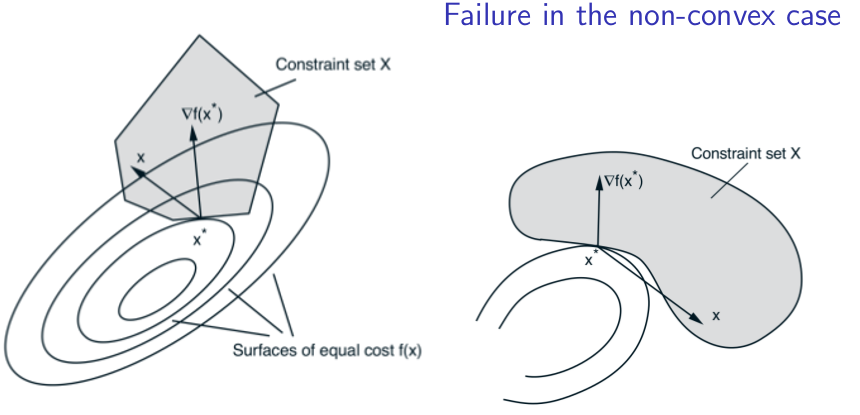
\includegraphics[width=\textwidth]{non_convex.png}
  \caption{Graphical representation of convex and non-convex set \label{fig:convex}}
\end{figure}

%%%%%%%%%%%%%%%%%%%%%%%%%%%%%%%%%%%%%%%%%%%%%%%%%%%%%%%%%%%
\begin{question}
  What is a projection on a convex set? Give the optimality condition and specialize the condition
  to the case where the convex set is a subspace.  Tell what are the properties of a subspace.
\end{question}
\begin{itemize}
\item $z$ is a fixed vector, find vector $x^*$ in a closed convex set X
\item $min_x f(x) = || x - z || ^2$
\end{itemize}

%%%%%%%%%%%%%%%%%%%%%%%%%%%%%%%%%%%%%%%%%%%%%%%%%%%%%%%%%%%
\begin{question}
  What is a feasible direction? Give an example. What is the general form of a feasible direction
  method? Also give an alternative form of the feasible direction based on a feasible vector
  \(\bar{x}\).
\end{question}
middle/end of pages slide 10 - start in interior and just take small steps $->$ we can ignore
constraint under these conditions
\begin{itemize}
\item Given a feasible vector $x$, a feasible
  direction at $x$ is a vector $d$ such that the
  vector $x + \alpha d$ is feasible for all sufficiently
  small $\alpha > 0$.
\item a feasable method generates starts at $x^0$ and generates multiple such points $x^{k+1}$
\end{itemize}

%%%%%%%%%%%%%%%%%%%%%%%%%%%%%%%%%%%%%%%%%%%%%%%%%%%%%%%%%%%
\begin{question}
  Explain the conditional gradient method and the projected gradient method.  What is different? For
  both methods draw a simple example showing how the feasible directions are computed.
\end{question}
\begin{itemize}
\item Conditional gradient solves subproblem with linear cost, gradient projection method solves
  quadratic cost fct
\item The conditional gradient method generates the point $\overline{x}^k$ by finding a feasible
  point which is furthest way from $x^k$ along the negative gradient direction $-\nabla f (x^k )$.

\end{itemize}
\begin{figure}[H]
  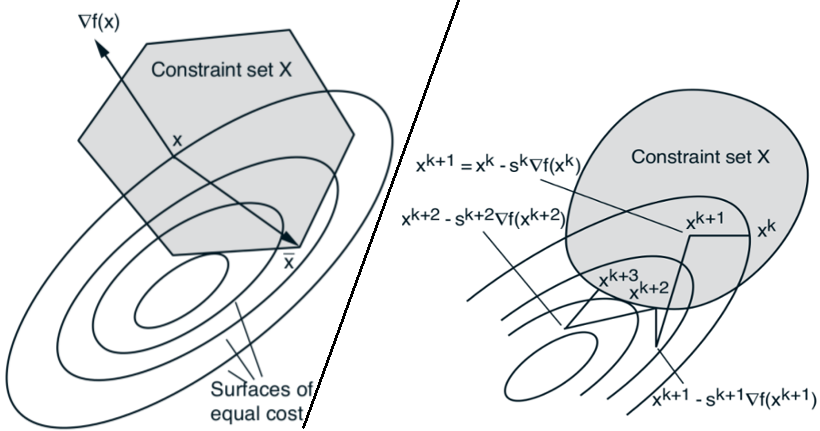
\includegraphics[width=\textwidth]{proj_desc.png}
  \caption{Graphical representation of conditional (left) and projective (right)
    method\label{fig:proj_desc}}
\end{figure}

%%%%%%%%%%%%%%%%%%%%%%%%%%%%%%%%%%%%%%%%%%%%%%%%%%%%%%%%%%%
\begin{question}
  What is the affine scaling method for solving an equality constrained LP? Show how the LP is
  solved based on solving a sequence of linearly constrained quadratic programs. Why can the
  inequality constraint be skipped?
\end{question}
\begin{itemize}
\item iterative method $x^{k+1} = x^k + \alpha^k (H^k)^{-1} (\texttt{big AHA formula})$
\item affine scaling: choose $H^k = (X^k)^{-2}$, $X^k = diag(x_1, ..., x_n)$ leads to
  $y^{k+1} = y^k + \alpha^k (AX^k A' )^{-1} b $, $\alpha^k$ ensures $x^{k+1} > 0$
\end{itemize}

%%%%%%%%%%%%%%%%%%%%%%%%%%%%%%%%%%%%%%%%%%%%%%%%%%%%%%%%%%%
\begin{question}
  What is the Lagrange multiplier theorem for equality constrained optimization problems? Draw a
  simple example and explain why the gradients of the constraint functions need to be linearly
  independent.
\end{question}
\begin{itemize}
\item Interpretation 1: The gradient of the cost function $\nabla f (x^*)$
  belongs to the subspace spanned by the gradients of the
  constraint functions $\nabla h_i (x^* )$
\item Interpretation 2: The cost gradient $\nabla f (x^* )$ is orthogonal to
  the subspace of first order feasible directions
\item for failure see figure~\ref{fig:ex1}. The Eigenvectors are lineary dependent, we loose one
  dimension and thus we can not optimize the problem (at least I think so)
\end{itemize}

%%%%%%%%%%%%%%%%%%%%%%%%%%%%%%%%%%%%%%%%%%%%%%%%%%%%%%%%%%%
\begin{question}
  Show how to solve the projection problem:
  \[
    \min_x \frac{1}{2} \enVert{x - y}^2
  \]
  Write down the Lagrangian, give the KKT conditions and show how the
problem is solved.
\end{question}

%%%%%%%%%%%%%%%%%%%%%%%%%%%%%%%%%%%%%%%%%%%%%%%%%%%%%%%%%%% 
\begin{question}
  Show how to compute the projection onto a half space:
  \[
    \min_x \frac{1}{2} \enVert{x-y}^2 \quad \text{s.t.} \quad \T{a}x = b
  \]
  Write down the Lagrangian, give the KKT conditions and show how the
  problem is solved.
\end{question}


\begin{figure}[H]
  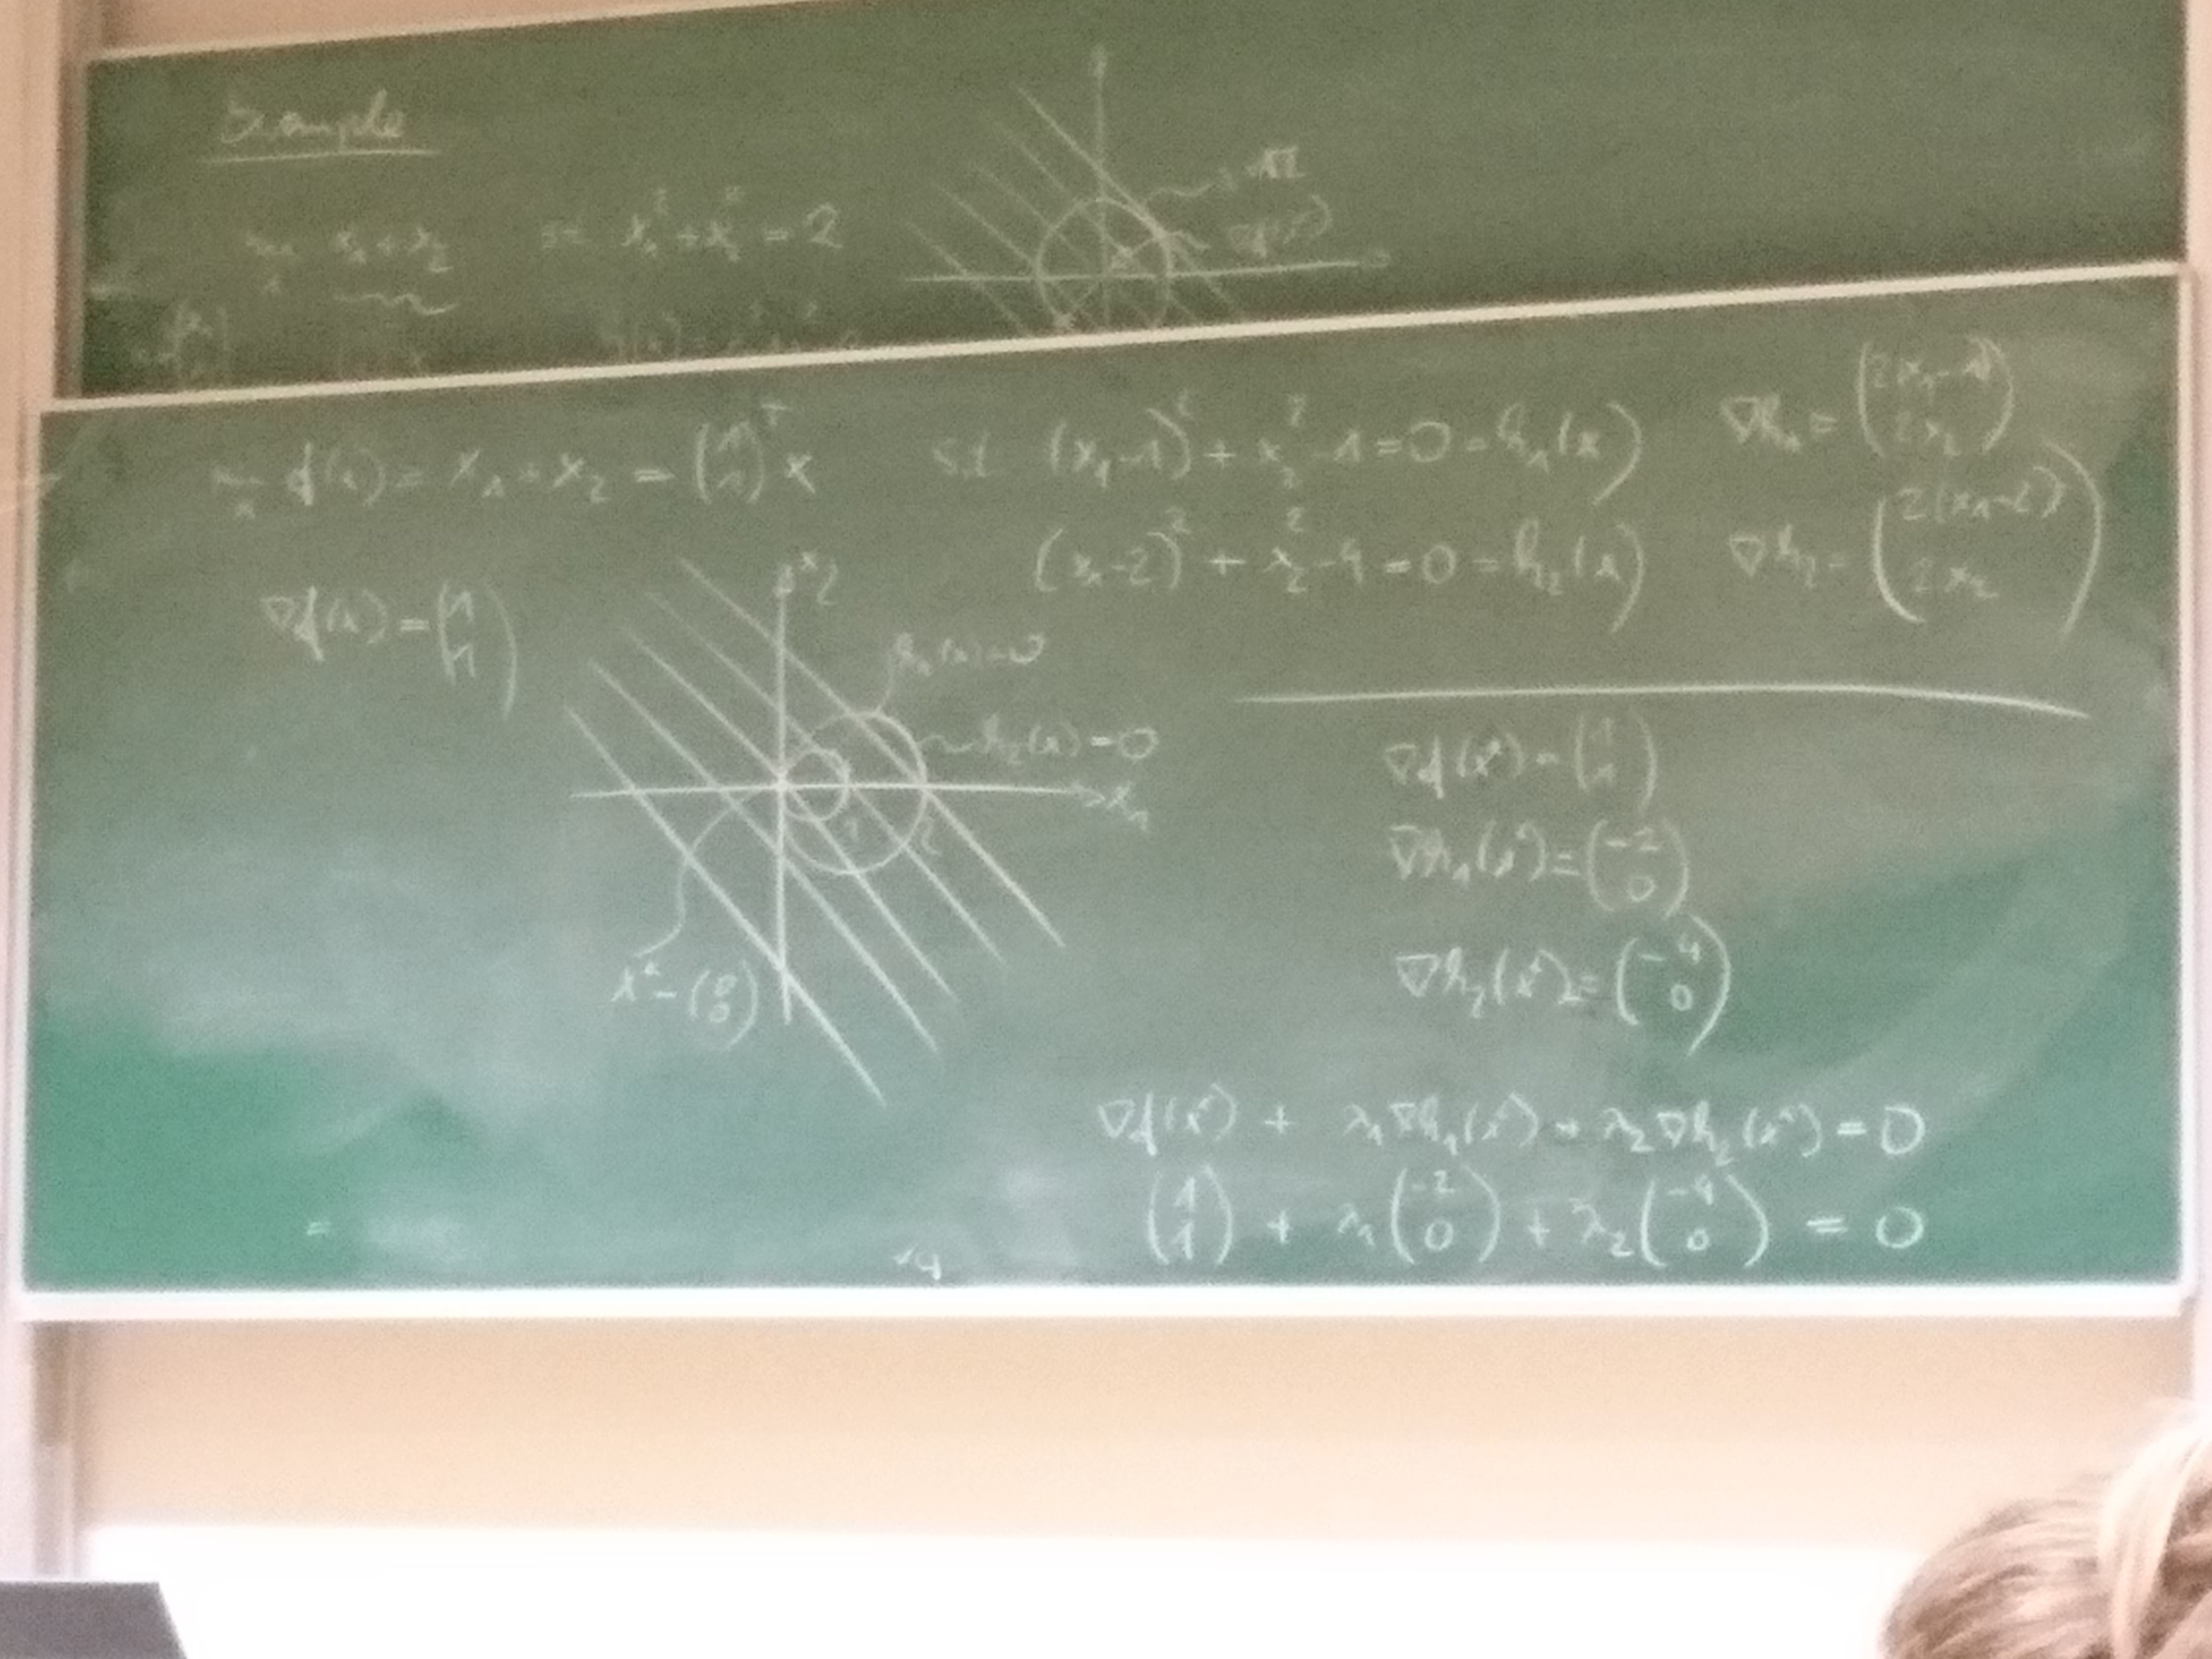
\includegraphics[width=\textwidth]{2017_01_24-ex1.jpg}
  \caption{Example1,  24.01.2017\label{fig:ex1}}
\end{figure}

\begin{figure}[H]
  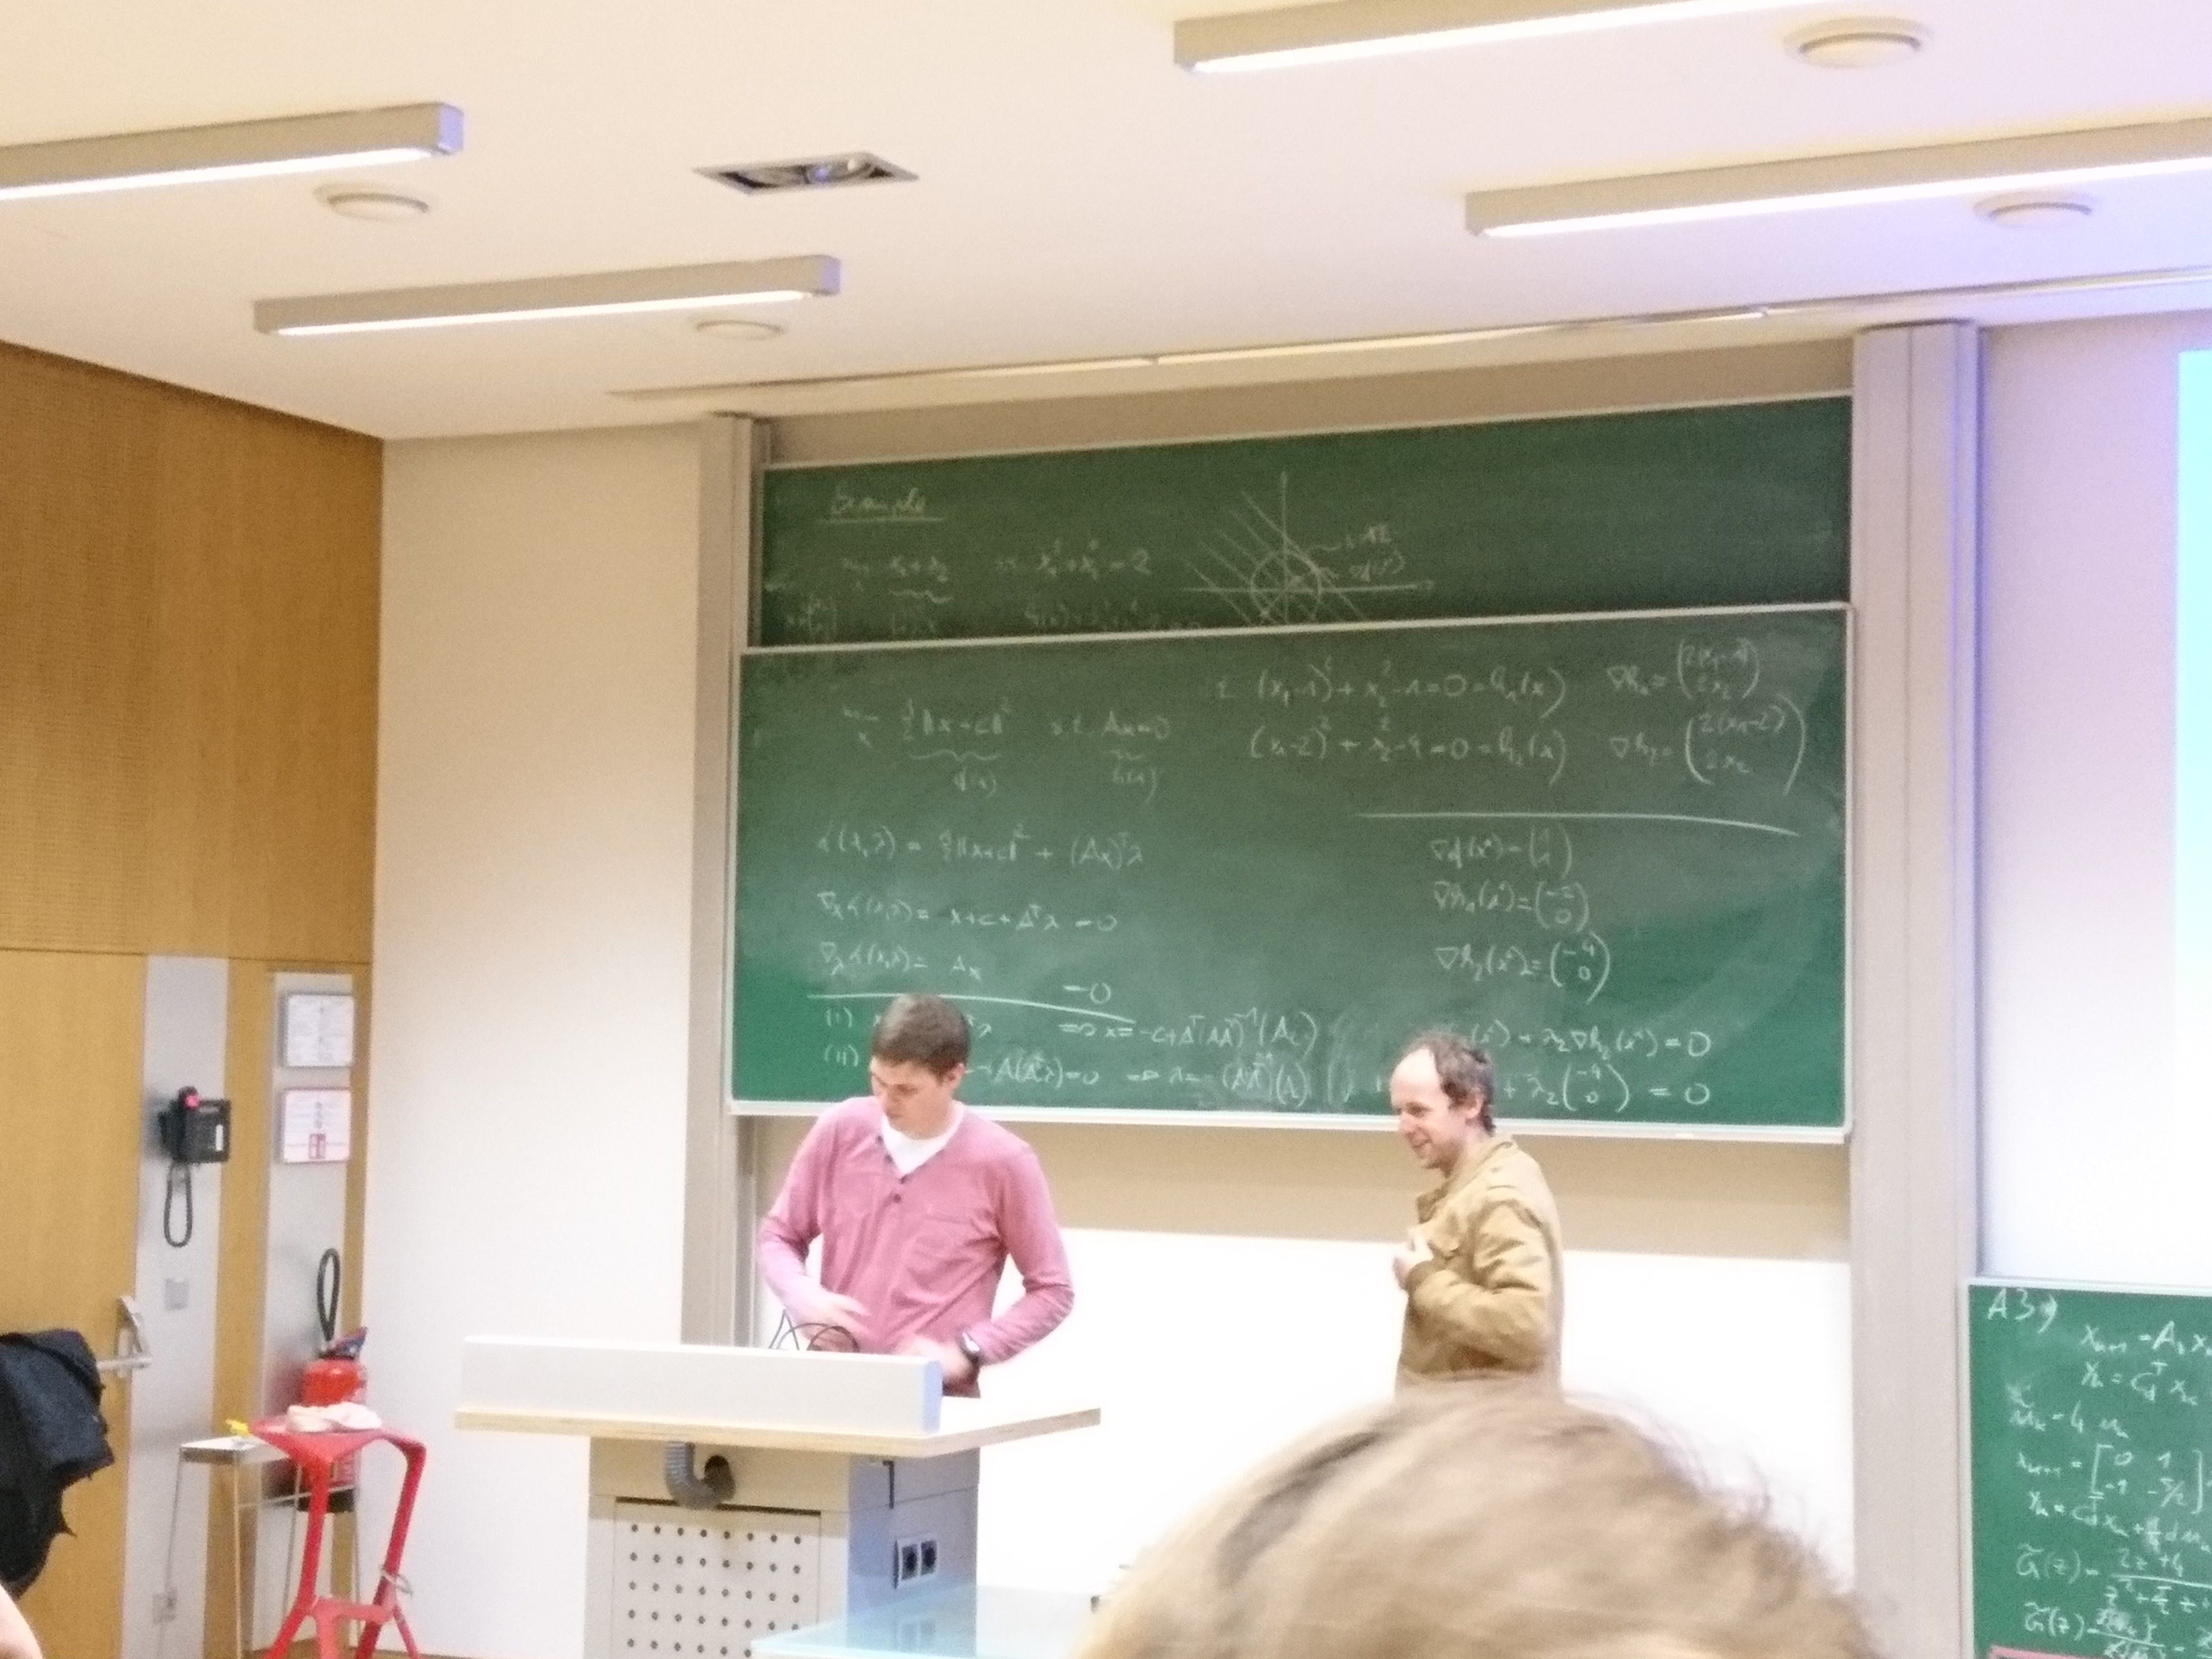
\includegraphics[width=\textwidth]{2017_01_24-ex2.jpg}
  \caption{Example 2,  24.01.2017\label{fig:ex2}}
\end{figure}
\end{document}
